%%
% 引言
% 引言是论文正文的开端,应包括毕业论文选题的背景、目的和意义;对国内外研究现状和相关领域中已有的研究成果的简要评述;介绍本项研究工作研究设想、研究方法或实验设计、理论依据或实验基础;涉及范围和预期结果等。要求言简意赅,注意不要与摘要雷同或成为摘要的注解。
%%

\chapter{引言}
\label{cha:introduction}

\section{问题背景}
\label{sec:background}
% What is the problem
% why is it interesting and important
% Why is it hards, why do naive approaches fails
% why hasn't it been solved before
% what are the key components of my approach and results, also include any specific limitations,do not repeat the abstract
%contribution

强化学习(Reinforcement Learning, RL)\cite{ReinforcementLearning2021} \cite{suttonReinforcementLearningIntroduction2018} 是机器学习(Machine Learning,  ML)领域的一部分。不同于监督学习,强化学习不需要带标签的学习样本, 而是利用奖励或惩罚智能体行为的方式间接设定学习目标, 是一种主动的学习方式 \cite{salvadorREINFORCEMENTLEARNINGLITERATURE2020}。 RL 的灵感来源于心理学中的行为主义理论,即有机体如何在环境给予的奖励或惩罚的刺激下,逐步形成对刺激的预期,产生能获得最大利益的习惯性行为\cite{ReinforcementLearning2021}。其它的机器学习例如监督学习和无监督学习,都是人为地设定明确的直接的学习目标,是一种被动的学习方式;相反地,强化学习是利用反馈机制,学习到合适的行为,是一种主动的学习方式。 从理论上讲,RL可以达到人工智能(Artificial General Intelligence, AGI)的状态,甚至可以达到人工智能(ASI)的状态,这是使智能体执行的最高目标。\cite{salvadorREINFORCEMENTLEARNINGLITERATURE2020}。

标准的强化学习中,有几个重要的概念:智能体(agent),环境(environment),状态(state),动作(action),奖励(reward)。考虑扫地机器人的场景:机器人通过在房间里移动和执行清扫动作,从而完成任务。如果有多个扫地机器人,如何挑选出“最好”的一个呢?我们可以计算每块地砖的清洁程度,设定合理的评分机制,从而挑选出得分最高的扫地机器人出来。如果从强化学习的角度看待这个问题,扫地机器人是智能体,房间里面的所有事物就是智能体所在的环境,智能体所在位置以及房间的形状、清洁程度就是改环境的状态,移动和执行清理动作是动作,而每块砖的清洁程度的增加量就是奖励,只是我们要训练出一个得分高的扫地机器人,而不是挑选出一个。现实中有很多这样的问题场景,例如棋盘游戏、电子游戏和自动驾驶等。我们抽象出强化学习的理论框架:智能体是完成任务的机器,它负责学习和决策,而智能体执行任务过程中应对的外部事物是环境。这些事务之间持续进行交互,智能体选择动作,环境对这些动作做出响应,呈现出新的状态。同时智能体获取一个奖励,这就是智能体在动作选择过程中最大化的目标。


\begin{figure}[h]
	\centering
	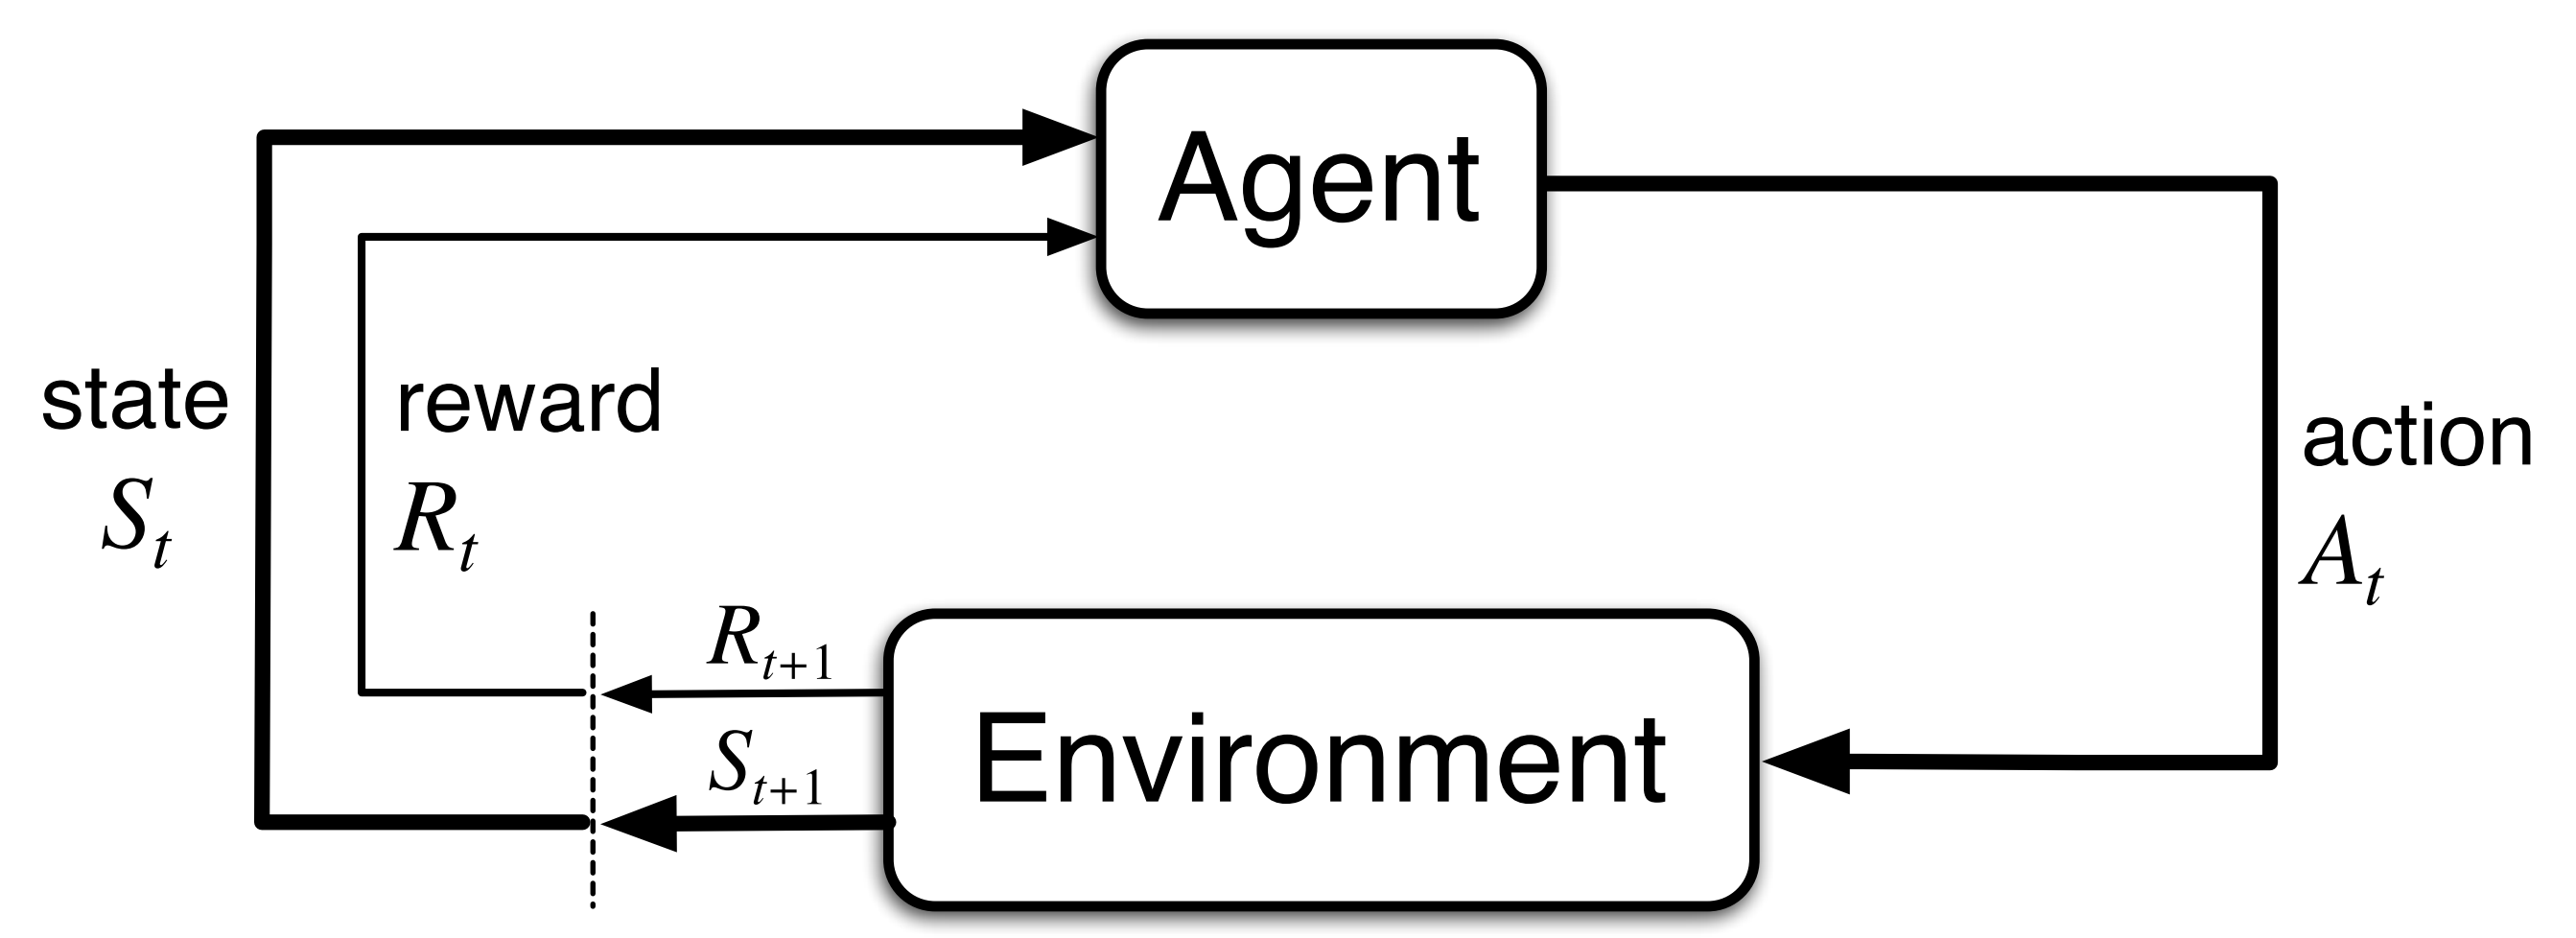
\includegraphics[width=0.9\textwidth]{image/chap01/interaction.png}
	\caption{智能体与环境交互过程\cite{suttonReinforcementLearningIntroduction2018}}
 	\label{fig:interaction-illustration}
\end{figure}

近些年来,强化学习在应用上取得巨大的成就。
RL中最令人兴奋的近期成功案例之一是DeepMind公司开发的AlphaGo \cite{silverMasteringGameGo2016} 和AlphaZero \cite{silverMasteringGameGo2017} 围棋程序。


AlphaZero可以玩国际象棋,围棋和其他游戏,相对于仅玩围棋的AlphaGo,它在性能和通用性方面都有改进。
这两个程序的性能均优于2020年所有竞争对手的计算机程序,并且比所有人的性能都要好得多。
这些程序在其他几个方面也很出色。特别是,他们学会了如何在没有人工指导的情况下玩游戏,而只是玩游戏而已。
此外,他们学习了如何快速演奏。
实际上,AlphaZero在几小时内就学会了比所有人类和计算机程序更好的下棋(必须说,借助强大的并行计算能力)。

作为人工智能领域的热门研究问题,深度强化学习自提出以来,就受到人们越来越多的关注.目前,深度 强化学习能够解决很多以前难以解决的问题,比如直接从原始像素中学习如何玩视频游戏和针对机器人问题学习 控制策略,深度强化学习通过不断优化控制策略,建立一个对视觉世界有更高层次理解的自治系统.其中,基于值函数和策略梯度的深度强化学习是核心的基础方法和研究重点.该文对这两类深度强化学习方法进行了系统的阐 述和总结,包括用到的求解算法和网络结构.首先,本文概述了基于值函数的深度强化学习方法,包括开山鼻祖深 度Q网络和基于深度Q网络的各种改进方法.然后介绍了策略梯度的概念和常见算法,并概述了深度确定性策略 梯度、信赖域策略优化和异步优势行动者评论家这三种基于策略梯度的深度强化学习方法及相应的一些改进方法.接着概述了深度强化学习前沿成果阿尔法狗和阿尔法元,并分析了后者和该文概述的两种深度强化学习方法 的联系.最后对深度强化学习的未来研究方向进行了展望.
对国内外研究现状和相关领域中已有的研究成果的简要评述。强化学习 \cite{suttonReinforcementLearningIntroduction2018}




\section{本文的论文结构与章节安排}
\label{sec:arrangement}

本文共分为六章,各章节内容安排如下:第一章引出 

第二章文献综述

第三章是算法

第四章是实验

第五章 结论

第六章是总结
